\chapter{Arhitektura i dizajn sustava}


\textbf{Arhitektura se može podijeliti na tri podsustava:}
\begin{itemize}
	\item \textit{Web poslužitelj}
	\item \textit{Web aplikacija}
	\item \textit{Baza podataka}
\end{itemize}

\emph{\textit{\textbf{Web preglednik}}} je program koji korisniku omogucuje pregled web-stranica i multimedijalnih sadrzaja vezanih uz njih. Svaki internetski preglednik je prevoditelj. Dakle, stranica je pisana u kodu koji preglednik nakon toga interpretira kao
nešto svakome razumljivo. Korisnik putem web preglednika šalje zahtjev web poslužitelju.

\emph{\textit{\textbf{Web poslužitelj}}} osnova je rada web aplikacije. Njegova primarna zadaća je komunikacija klijenta s aplikacijom. Komunikacija se odvija preko HTTP (engl. Hyper
Text Transfer Protocol) protokola, sto je protokol u prijenosu informacija na webu.
Poslužitelj je onaj koji pokreće web aplikaciju te joj prosljeđuje zahtjev.

Korisnik koristi \emph{\textit{\textbf{web aplikaciju}}} za obrađivanje željenih zahtijeva. Web aplikacija
obrađuje zahtjev te ovisno o zahtjevu, pristupa bazi podataka nakon cega preko
poslužitelja vraća korisniku odgovor u obliku HTML dokumenta vidljivog u web
pregledniku

Programski jezik kojeg smo odabrali za izradu naše web aplikacije je Java zajedno s Spring Boot radnim okvirom te JSP obrascima za frontend. Odabrano razvojno okruženje je InteliJ IDEA. Arhitektura sustava temeljiti će se na MVC (Model-View-Controller) konceptu. MVC koncept podržan je od strane Spring Boot radnog okvira i kao takav ima gotove predloške koji nam olakšavaju razvoj web aplikacije.

Karakteristika MVC koncepta je nezavisan razvoj pojedinih dijelova aplikacije
što za posljedicu ima jednostavnije ispitivanje kao i jednostavno razvijanje i dodavanje novih svojstava u sustav.

MVC koncept sastoji se od:
\begin{itemize}
	\item \textbf{Model} -  Središnja komponenta sustava. Predstavlja dinamičke strukture podataka, neovisne o korisnickom sučelju. Izravno upravlja podacima, logikom
	i pravilima aplikacije. Takoder prima ulazne podatke od Controllera
	\item \textbf{View} - Bilo kakav prikaz podataka, poput rasporeda. Mogući su različiti prikazi iste informacije poput grafičkog i tabličnog prikaza podataka.
	\item \textbf{Controller} - Prima ulaze i prilagođava ih za prosljeđivanje Modelu ili Viewu. Upravlja korisničkim zahtjevima i temeljem njih izvodi daljnju interakciju s ostalim elementima sustava.
\end{itemize}





\pagebreak

\section{Baza podataka}

Kao implementaciju baze podataka u ovome projektu odabrali smo
postgreSQL RDMS. Baza podataka se sastoji od tablica koje
predstavljaju entitete u Kampu mlade nade. Za potrebe naseg sustava koristit cemo relacijsku bazu podataka koja svojom strukturom olaksava modeliranje stvarnog svijeta. Gradivna jedinka baze je relacija, odnosno tablica koja je definirana svojim imenom i skupom atributa. Zadaca baze podataka je brza i jednostavna pohrana, izmjena i dohvat podataka za daljnju obradu. Baza podataka ove aplikacije sastoji se od entiteta koji su opisanu u nastavku.
\vspace{5mm} %5mm vertical space		
\subsection{Opis tablica}
\vspace{5mm} %5mm vertical space		
\textbf{Person}
\\ Ovaj entitet modelira osobu koja se prijavljuje na kamp, bilo kao sudionik ili kao animator. Sadrži atribute ID osobe, nickname, motivational letter, birthday, email, password, surname, name, telephone, accepted i nickhash. S entitetom Prijava u vezi je tipa One-to-One. Također služi kao nad-entitet za entitete Sudionk i Animator, koji nasljeđuju sve atribute. Osim toga, svaka osoba povezana je Many-to-One vezom sa entitetom Komentar.

\begin{longtabu} to \textwidth {|X[6, l]|X[6, l]|X[20, l]|}

\hline \multicolumn{3}{|c|}{\textbf{Osoba}}
\\[3pt] \hline
\endfirsthead

\hline
\endlastfoot

\cellcolor{LightGreen}ID osobe & VARCHAR & Jedinstveni identifikator sudionika.
\\ \hline
motivational letter & VARCHAR & Motivacijsko pismo osobe.
\\ \hline
birthday & DATE & Datum i godina rođenja osobe.
\\ \hline
name & VARCHAR & Ime osobe.
\\ \hline
surname & VARCHAR & Prezime osobe.
\\ \hline
email & VARCHAR & Email osobe.
\\ \hline
telephone & VARCHAR & Telefon osobe.
\\ \hline
nickname & VARCHAR & Korisničko ime osobe.
\\ \hline
nickHash & VARCHAR & Hash vrijednost korisničkog imena


\end{longtabu}
\pagebreak
\textbf{Participant}
\\ Ovaj entitet sadržava sve važne informacije o sudioniku kampa. Preuzima sve atribute nad-entiteta Osobe te uz to sadrži još jedan atribut - contact, koji predstavlja kontakt skrbnika za sudionike mlađe od 18 godina. Ovaj entitet je u vezi One-to-Many s entitom Grupa, te ima dodatni vlastiti atribut Korisničko ime. Entitet modelira osobu koja prisustvuje kampu.

\begin{longtabu} to \textwidth {|X[6, l]|X[6, l]|X[20, l]|}

\hline \multicolumn{3}{|c|}{\textbf{Sudionik}}
\\[3pt] \hline
\endfirsthead

\hline
\endlastfoot

contact \newline & VARCHAR & Opcionalni atribut, broj mobitela skrbnika djeteta mlađeg od 18 godina.
\\ \hline
\cellcolor{LightBlue}
ID osobe & INT & ID osobe koja se prijavila na kamp kao sudionik.\newline
\\ \hline
\cellcolor{LightBlue}
ID grupe & VARCHAR & ID grupe kojoj je osoba pridružena.

\end{longtabu}
\vspace{5mm} %5mm vertical space		
\textbf{Animator}
\\ Ovaj entitet sadržava sve važne informacije o animatoru kampa. Preuzima sve atribute nad-entiteta Osobe. Ovaj entitet je u vezi Many-to-Many s entitom Aktivnost u vremenu, te ima dodatni vlastiti atribut Korisničko ime. Entitet modelira osobu koja je zadužena za provođenje aktivnosti u kampu.

\begin{longtabu} to \textwidth {|X[6, l]|X[6, l]|X[20, l]|}

\hline \multicolumn{3}{|c|}{\textbf{Animator}}
\\[3pt] \hline
\endfirsthead

\hline
\endlastfoot

\cellcolor{LightBlue}
ID aktivnosti u vremenu \newline & VARCHAR & Jedinstveni identifikator aktivnosti u vremenu kojoj je pridružen animator.
\\ \hline
\cellcolor{LightBlue}
ID osobe & INT & ID osobe koja se prijavila na kamp kao animator.\newline


\end{longtabu}
\pagebreak

\textbf{Comment}
\\
Ovaj entitet modelira komentare koje ostavljaju sudionici i animatori po završetku kampa. Sadrži atribute ID komentara, grade, description te ID osobe. Entitet je u vezi One-to-Many sa Osobom i One-to-Many s Aktivnosti.

\begin{longtabu} to \textwidth {|X[6, l]|X[6, l]|X[20, l]|}

\hline \multicolumn{3}{|c|}{\textbf{Komentar}}
\\[3pt] \hline
\endfirsthead

\hline
\endlastfoot

\cellcolor{LightGreen}
ID komentara & VARCHAR & Jedinstveni identifikator komentara koji je osoba ostavila za aktivnost.\newline
\\ \hline
\cellcolor{LightGreen}
grade & INT & Ocjena aktivnosti.
\\ \hline
description & VARCHAR & Komentar odnosno kratki dojam o aktivnosti.

\\ \hline
\cellcolor{LightGreen}
ID osobe & VARCHAR & ID osobe koja je komentirala aktivnost.

\end{longtabu}
\vspace{5mm} %5mm vertical space		

\textbf{Activity}
\\
Ovaj entitet predstavlja aktivnosti koje kamp Mlade Nade nudi svojim polaznicima. Aktivnost se sastoji od sljedećih atributa: ID aktivnosti, name, description, duration, type, ID ktivnosti u vremenu, ID komentara. Povezana je Many-to-One vezom s entitetom Komentar, te vezom Many-to-One s Aktivnosti u vremenu.

\begin{longtabu} to \textwidth {|X[6, l]|X[6, l]|X[20, l]|}

\hline \multicolumn{3}{|c|}{\textbf{Aktivnost}}
\\[3pt] \hline
\endfirsthead

\hline
\endlastfoot

\cellcolor{LightGreen}
ID aktivnosti & VARCHAR & Jedinstveni ID aktivnosti.
\\ \hline
name & TIME & Ime aktivnosti.
\\ \hline
description & VARCHAR & Jedinstveni opis aktivnosti.

\\ \hline
duration & VARCHAR & Trajanje aktivnosti.

\\ \hline
type & VARCHAR & Tip aktivnosti.

\\ \hline
ID activity in time & VARCHAR & ID aktivnosti u vremenu, preciznije to je konkretna implementacija Aktivnosti.

\\ \hline
ID comment & VARCHAR & ID komentara koji su osobe postavile na aktivnosti.

\end{longtabu}
\vspace{5mm} %10mm vertical space		
\textbf{Activity in time}
\\
Ovaj entitet predstavlja aktivnost u kampu koja se odvija u specifičnom vremenu, odnosno predstavlja aktivnost koju sudionici, animatori i organizatori vide u svojim rasporedima. Od atributa ima ID aktivnosti u vremenu, end i start. Primarni ključ ovog entiteta je ID aktivnosti u vremenu. Entitet je u One-to-Many vezi s Aktivnosti, Many-to-Many vezi s Animatorom te Many-to-Many vezom s Grupom.

\begin{longtabu} to \textwidth {|X[6, l]|X[6, l]|X[20, l]|}

\hline \multicolumn{3}{|c|}{\textbf{Aktivnost u vremenu}}
\\[3pt] \hline
\endfirsthead

\hline
\endlastfoot

\cellcolor{LightGreen}
start & DATE & Početak aktivnosti.
\\ \hline
\cellcolor{LightGreen}
end & DATE & Kraj aktivnosti.
\\ \hline
\cellcolor{LightGreen}
ID aktivnosti u vremenu & VARCHAR & Ime aktivnosti.

\\ \hline
\cellcolor{LightBlue}
ID grupe & VARCHAR & ID grupe koja sudjeluje na trenutnoj aktivnosti.

\\ \hline
\cellcolor{LightBlue}
Korisničko ime & VARCHAR & Korisničko ime animatora koji je zadužen za tu aktivnost.

\end{longtabu}
\textbf{Group}
\\
Ovaj entitet modelira grupe sudionika na kampu. O broju i sadržaju grupa brine se organizator na početku kampa. Entitet sadrži atribute ID grupe, ime sudionika i ID aktivnosti u vremenu. Povezan je Many-to-One vezom sa Sudionikom te Many-to-Many vezom sa Aktivnosti u vremenu.

\begin{longtabu} to \textwidth {|X[6, l]|X[6, l]|X[20, l]|}

\hline \multicolumn{3}{|c|}{\textbf{Grupa}}
\\[3pt] \hline
\endfirsthead

\hline
\endlastfoot

\cellcolor{LightGreen}
ID grupe & VARCHAR & Jedinstveni ID grupe.
\\ \hline
\cellcolor{LightBlue}
Ime sudionika & VARCHAR & Ime sudionika koji pripada grupi.

\\ \hline
\cellcolor{LightBlue}
ID aktivnosi u vremenu & VARCHAR & ID aktivnosti kojoj određena pripada u nekom vremenu.


\end{longtabu}
\pagebreak
\textbf{Organizator}
\\
Ovaj entitet modelira organizatora kampa. Sadrži atribute nickname i password. On ima najveće ovlasti od svih te nije povezan niti s jednim od ostalih entiteta.

\begin{longtabu} to \textwidth {|X[6, l]|X[6, l]|X[20, l]|}

\hline \multicolumn{3}{|c|}{\textbf{Grupa}}
\\[3pt] \hline
\endfirsthead

\hline
\endlastfoot

\cellcolor{LightGreen}
nickname & VARCHAR & Korisničko ime organizatora.
\\ \hline
\cellcolor{LightBlue}
password & VARCHAR & Password organizatora.

\end{longtabu}
\pagebreak
\subsection{Dijagram baze podataka}
\begin{figure}[H]
	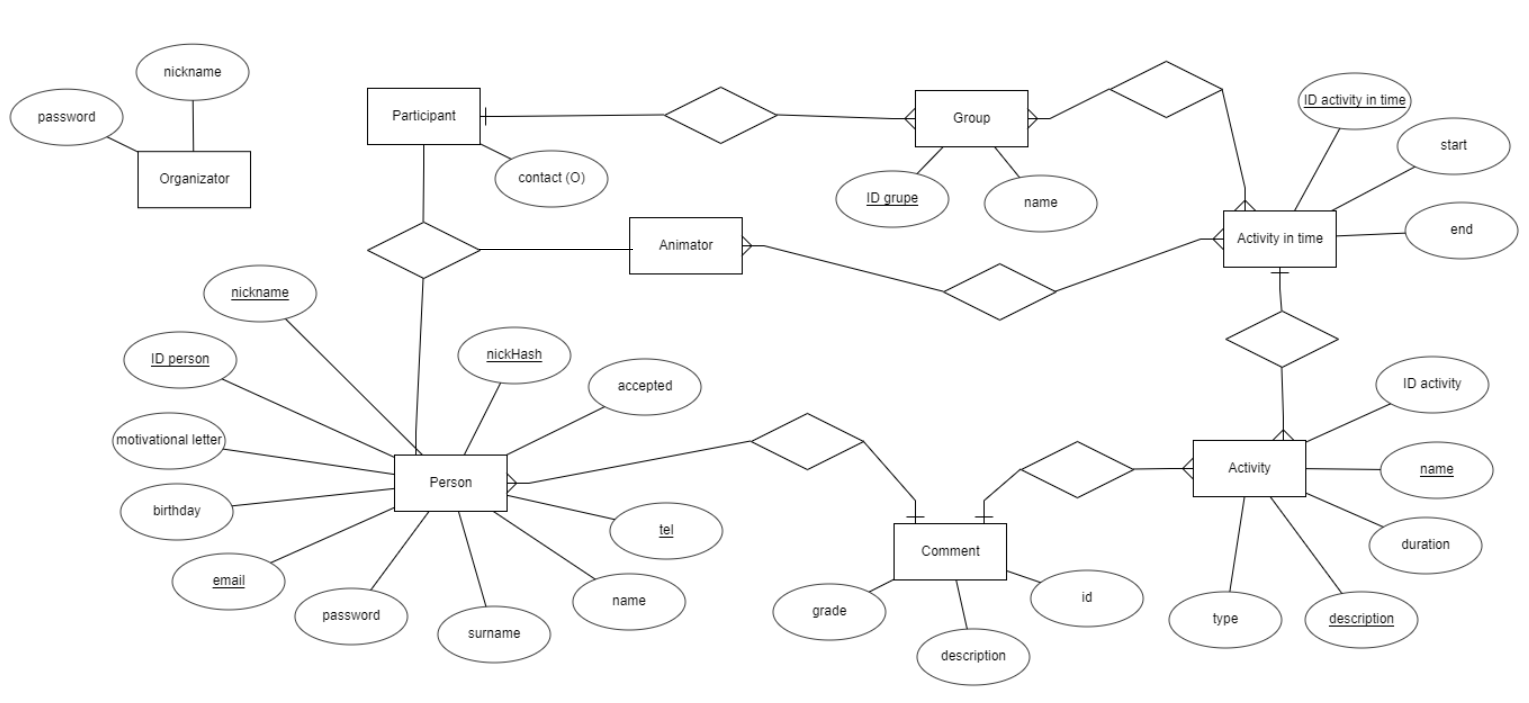
\includegraphics[scale=0.4]{dijagrami/erDijagram.PNG} %veličina slike u odnosu na originalnu datoteku i pozicija slike
	\centering
	\caption{ER dijagram baze podataka}
	\label{fig:promjene}
\end{figure}

\begin{figure}[H]
	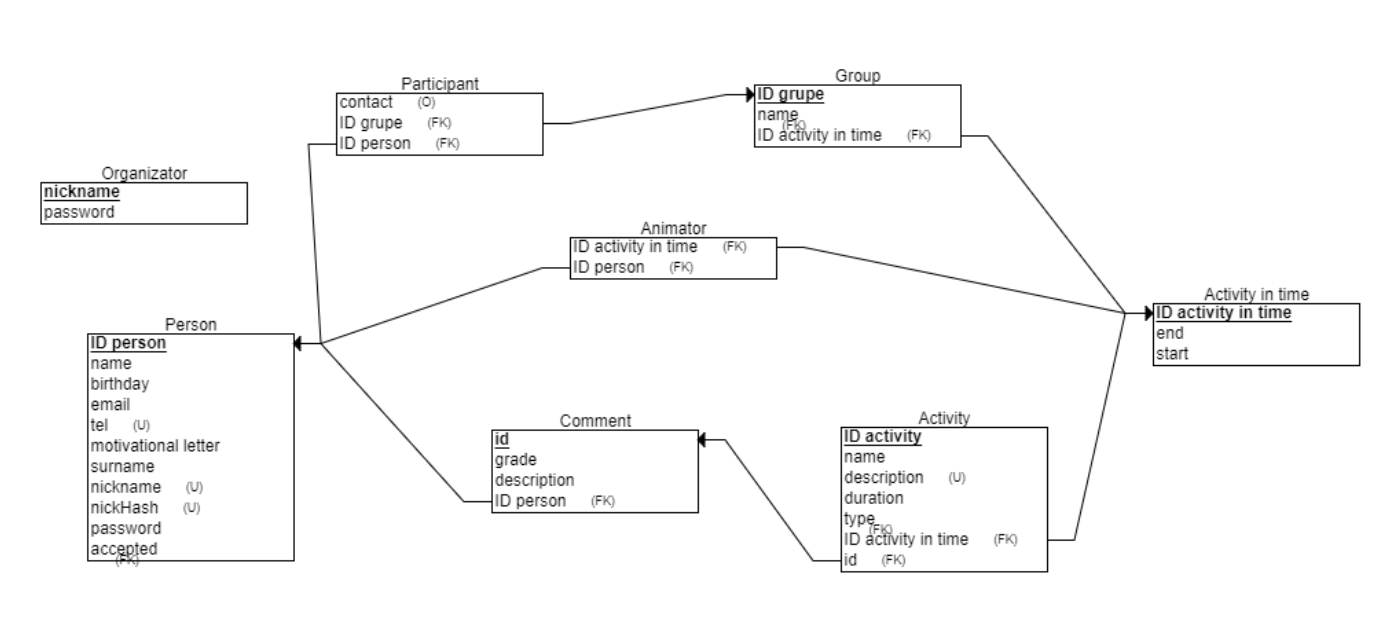
\includegraphics[scale=0.6]{dijagrami/rsDijagram.PNG} %veličina slike u odnosu na originalnu datoteku i pozicija slike
	\centering
	\caption{Relacijska shema baze podataka}
	\label{fig:promjene}
\end{figure}

\eject


\section{Dijagram razreda}

\begin{figure}[H]
	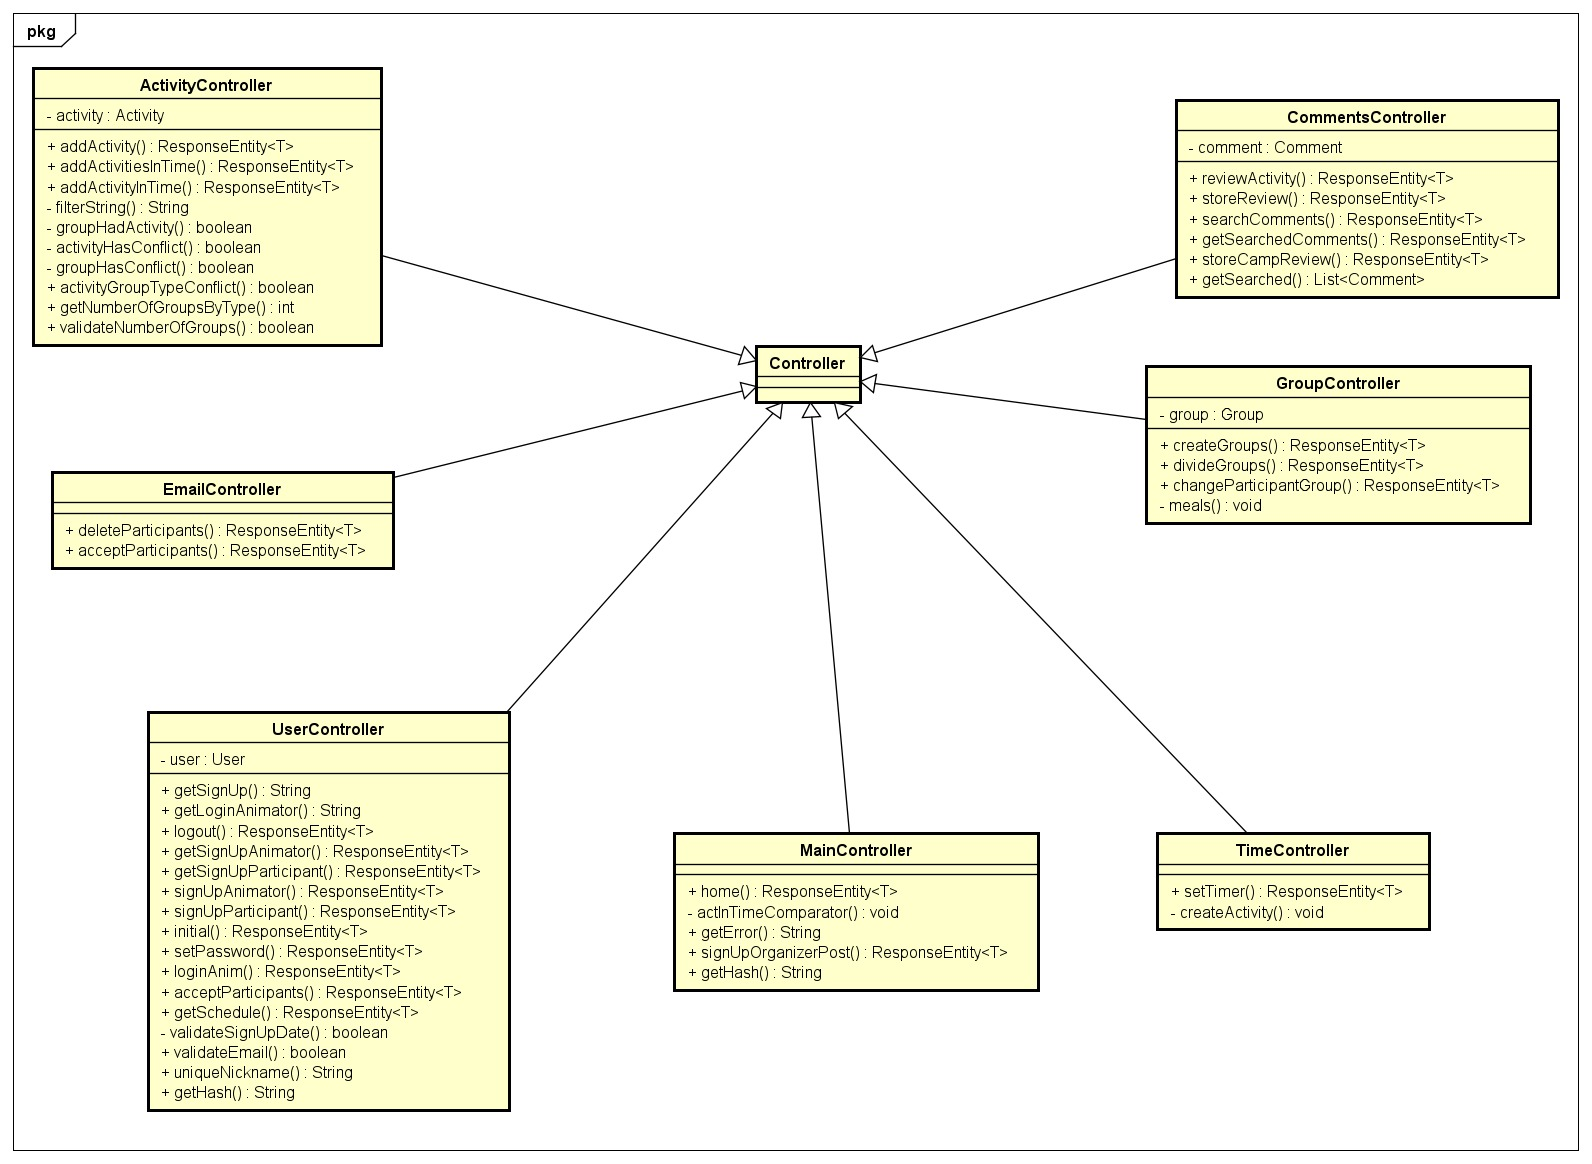
\includegraphics[scale=0.3]{dijagrami/Controllers.png} %veličina slike u odnosu na originalnu datoteku i pozicija slike
	\centering
	\caption{Controlleri}
	\label{fig:promjene}
\end{figure}

\begin{figure}[H]
    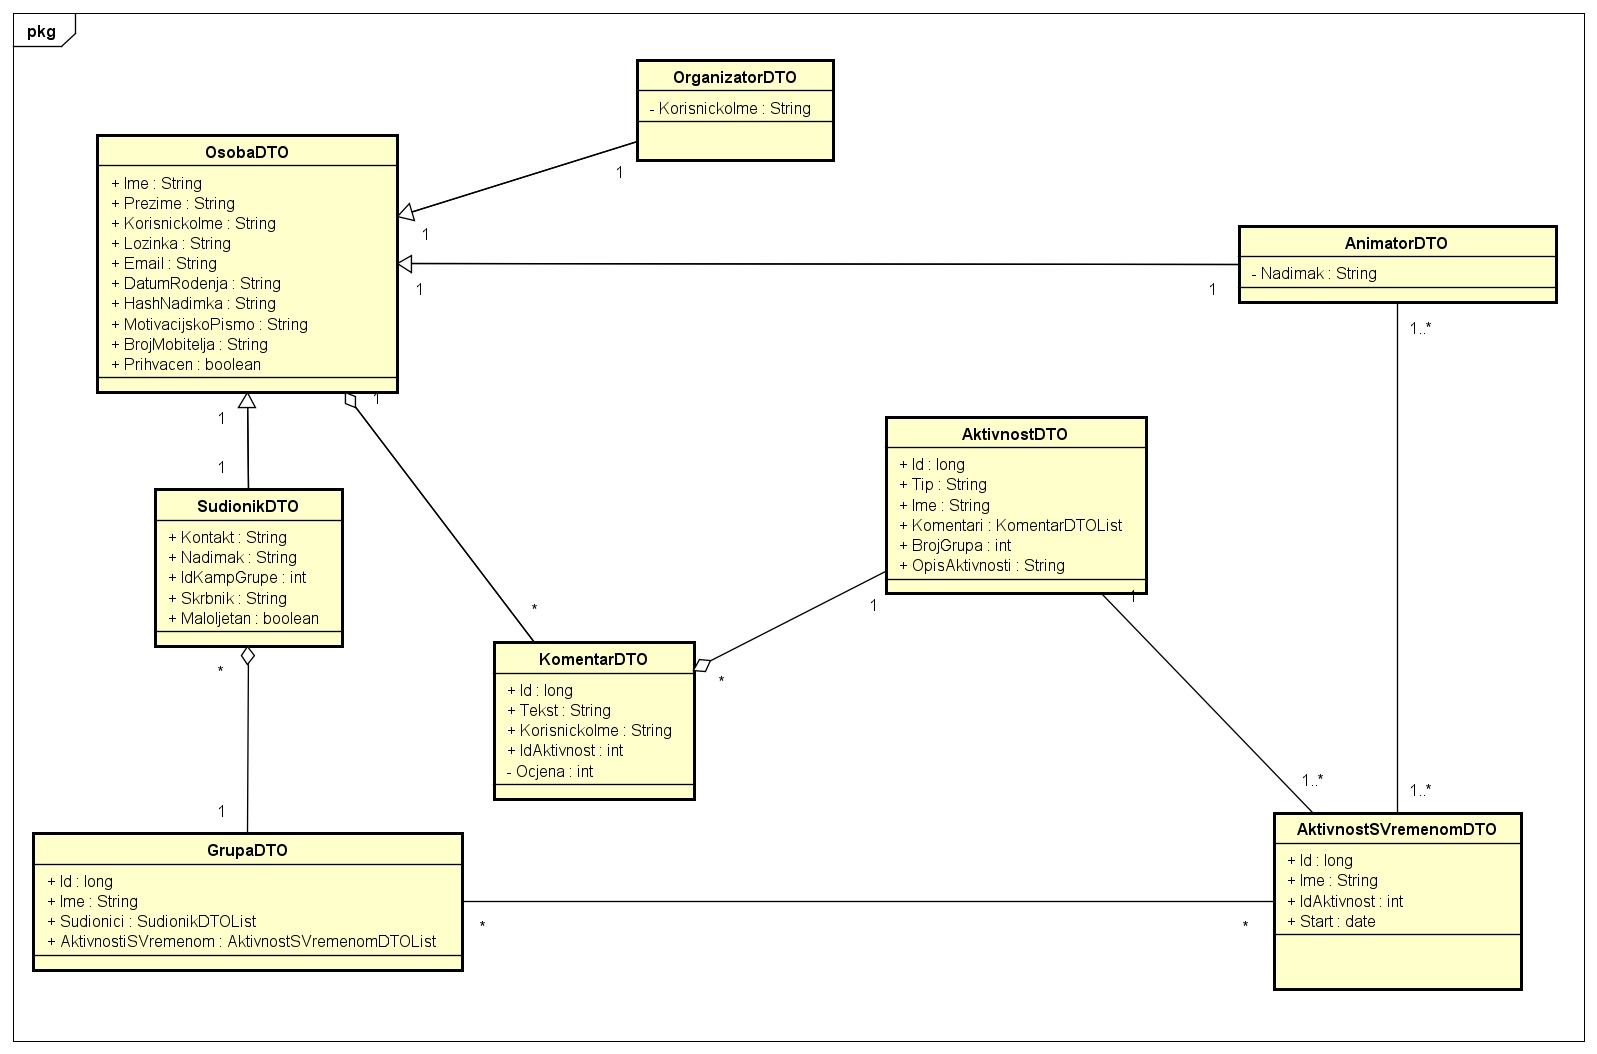
\includegraphics[scale=0.3]{dokumentacija/dijagrami/dto.jpeg} %veličina slike u odnosu na originalnu datoteku i pozicija slike
	\centering
	\caption{DTO}
	\label{fig:promjene}
\end{figure}


\begin{figure}[H]
	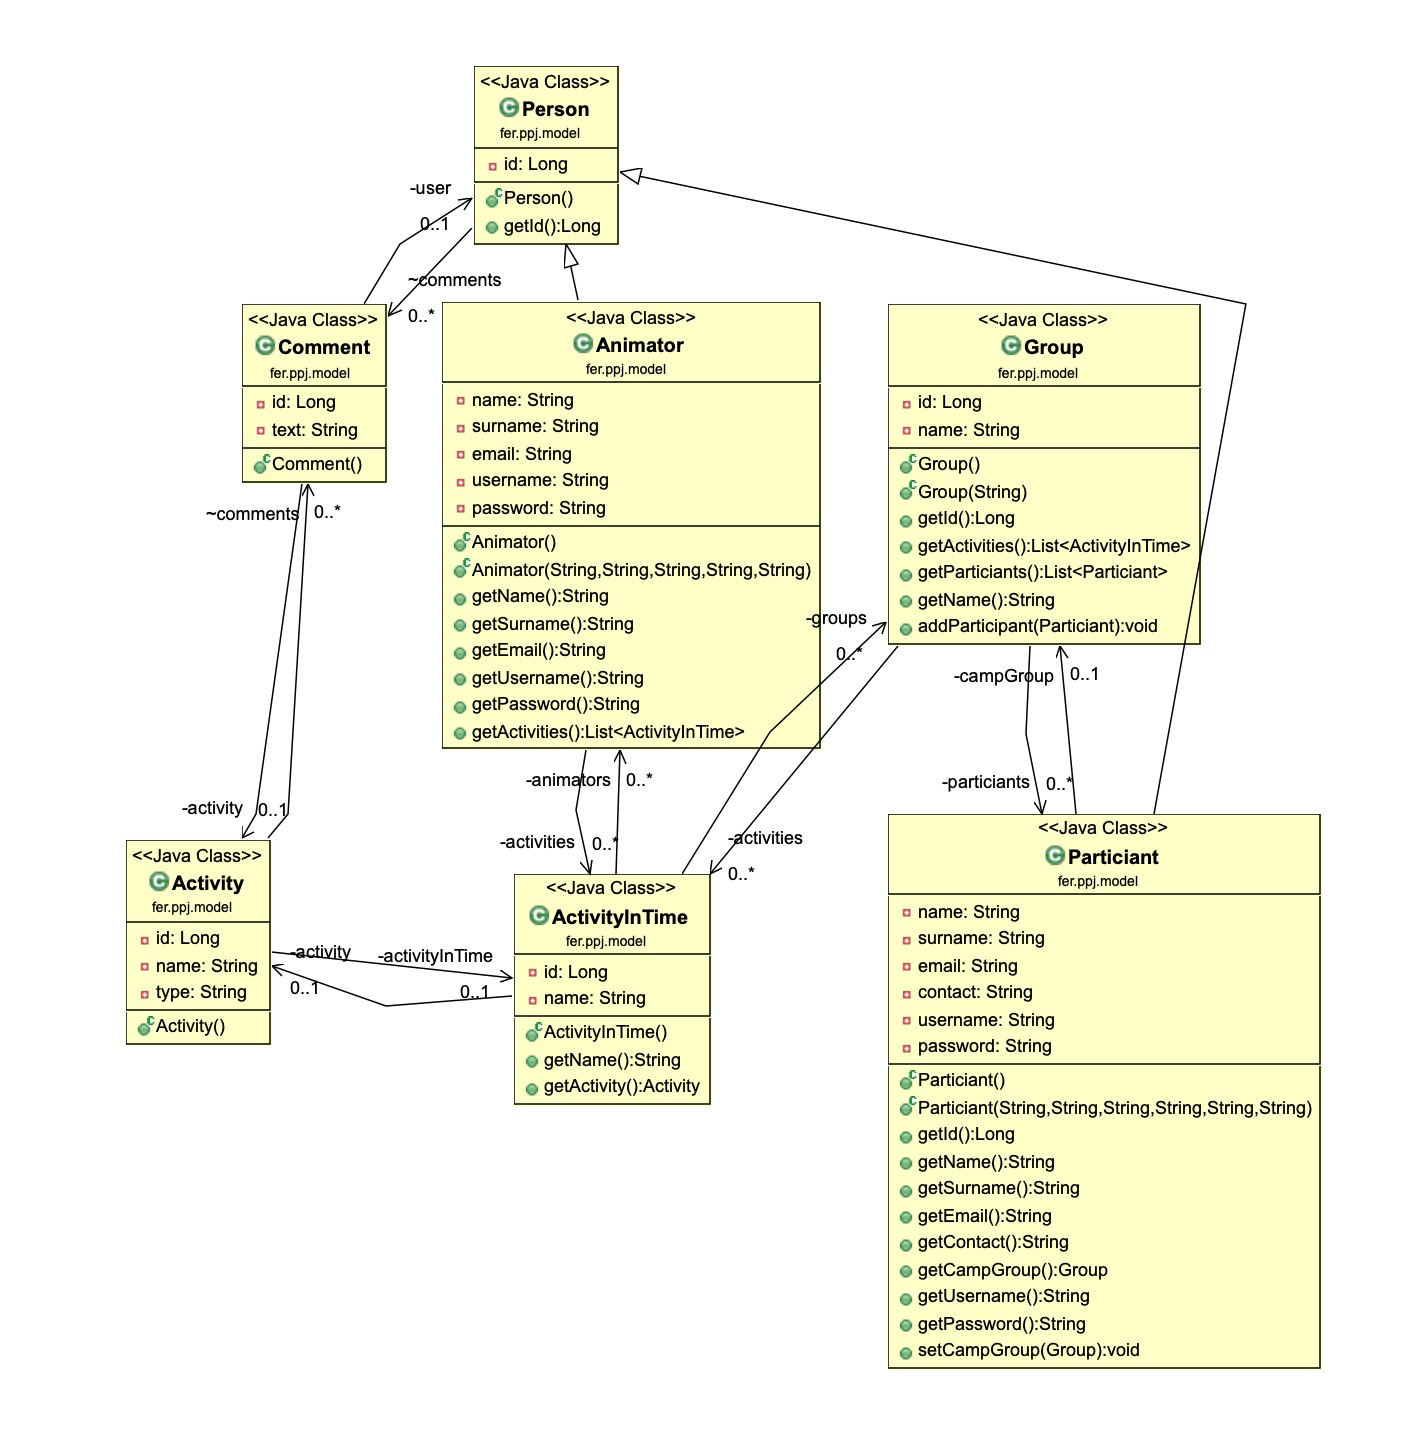
\includegraphics[scale=0.35]{dijagrami/dijagramRazreda.jpeg} %veličina slike u odnosu na originalnu datoteku i pozicija slike
	\centering
	\caption{Dijagram razreda}
	\label{fig:promjene}
\end{figure}





\eject

\section{Dijagram stanja}

\begin{figure}[H]
	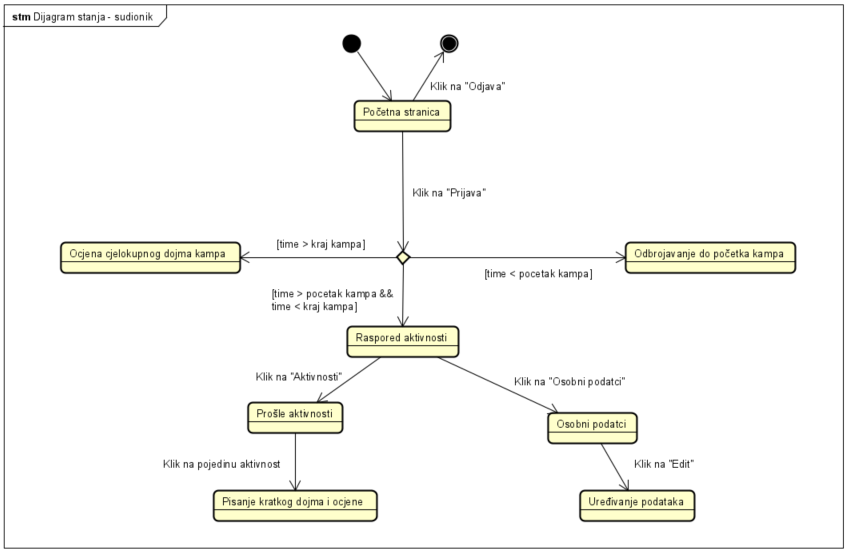
\includegraphics[scale=0.9]{dokumentacija/dijagrami/state-sudionik.PNG} 
	\centering
	\caption{DIjagram stanja sudionika}
	\label{fig:promjene}
\end{figure}

\begin{figure}[H]
	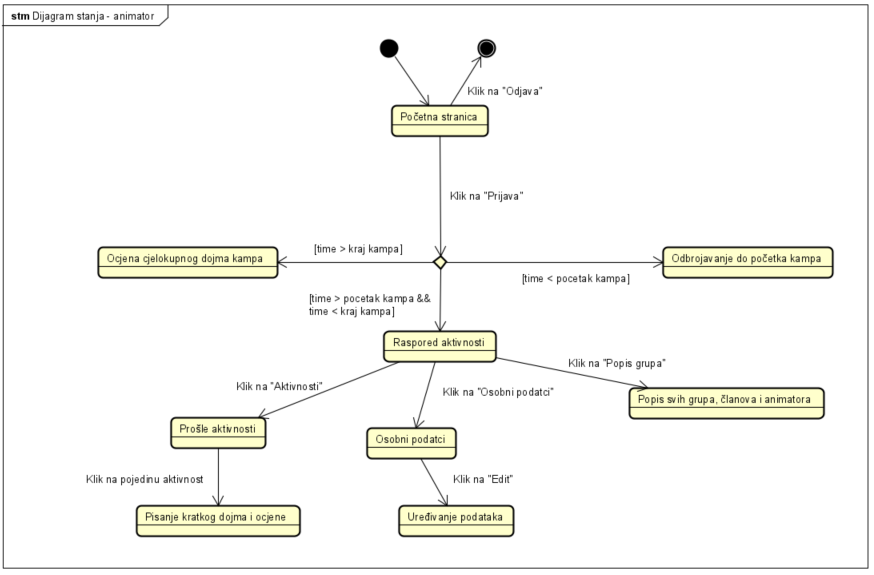
\includegraphics[scale=0.9]{dokumentacija/dijagrami/state-animator.PNG} 
	\centering
	\caption{DIjagram stanja animatora}
	\label{fig:promjene}
\end{figure}

\begin{figure}[H]
	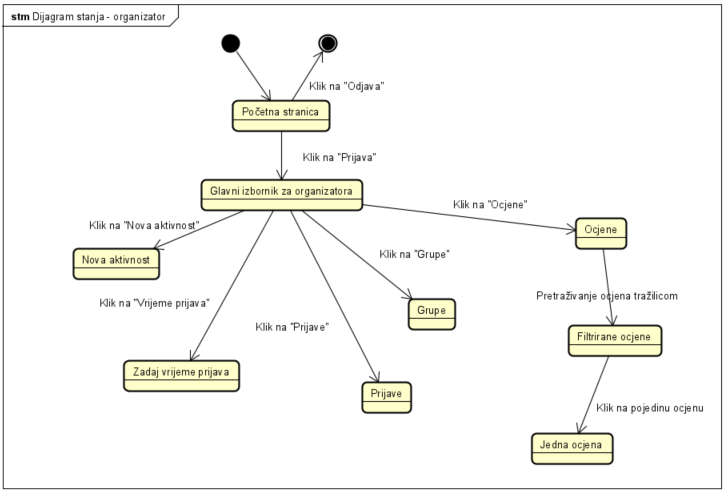
\includegraphics[scale=0.9]{dokumentacija/dijagrami/state-organizator.PNG} 
	\centering
	\caption{DIjagram stanja organizatora}
	\label{fig:promjene}
\end{figure}

\eject

\section{Dijagram aktivnosti}

\begin{figure}[H]
	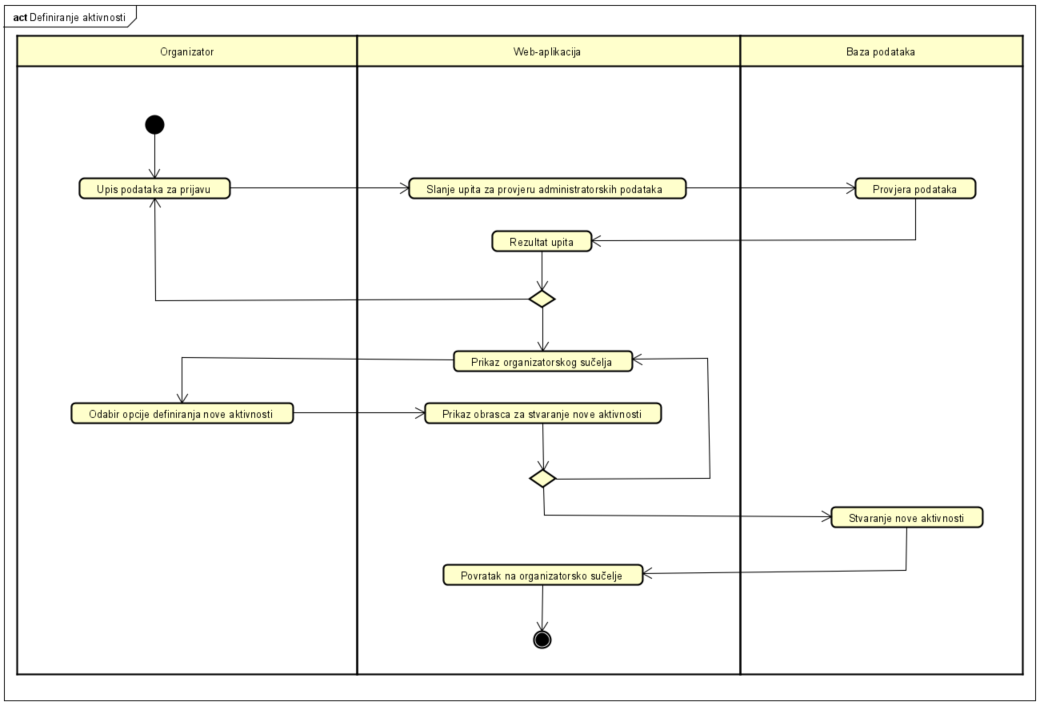
\includegraphics[scale=0.75]{dokumentacija/dijagrami/activity-definiranjeAktivnosti.PNG} 
	\centering
	\caption{Definiranje aktivnosti}
	\label{fig:promjene}
\end{figure}

\begin{figure}[H]
	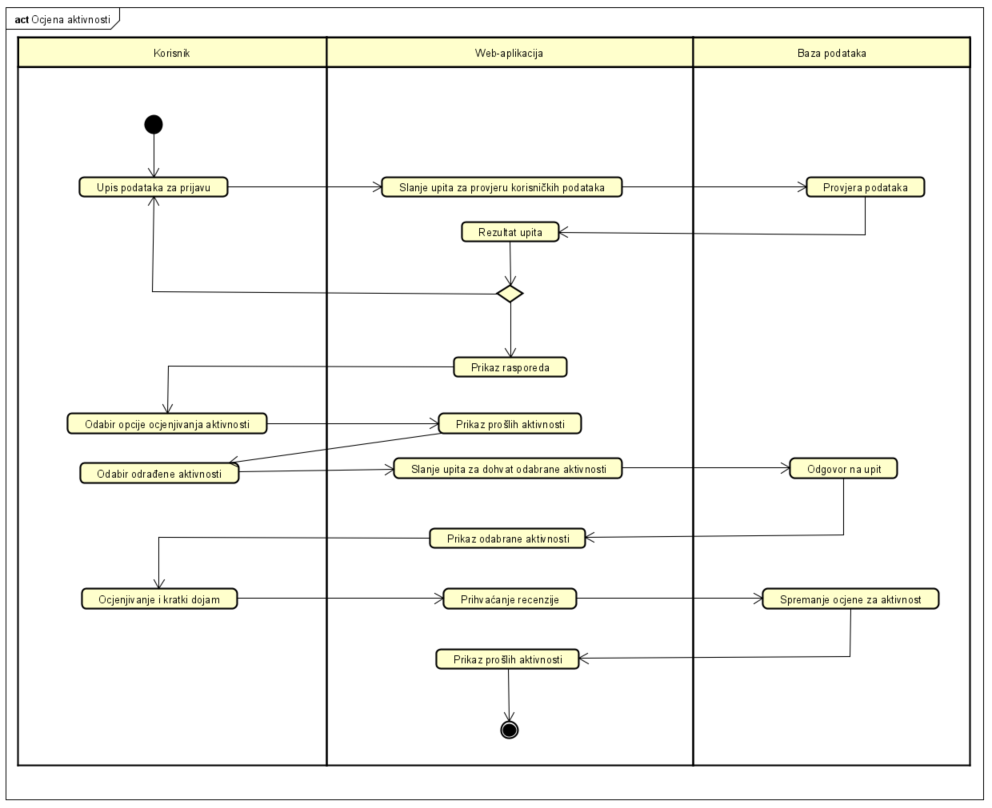
\includegraphics[scale=0.75]{dokumentacija/dijagrami/activity-ocjenaAktivnosti.PNG} 
	\centering
	\caption{Ocjena aktivnosti}
	\label{fig:promjene}
\end{figure}

\begin{figure}[H]
	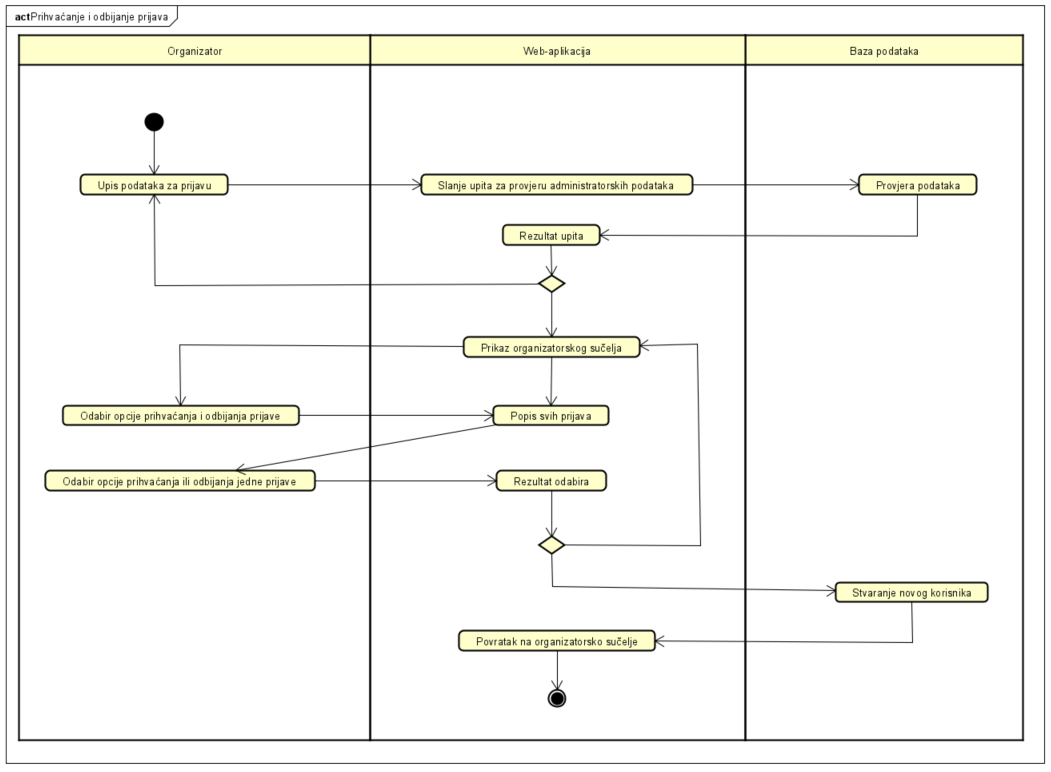
\includegraphics[scale=0.75]{dokumentacija/dijagrami/activity-prihvacanjeOdbijanjePrijava.PNG} 
	\centering
	\caption{Prihvaćanje i odbijanje prijava korisnika}
	\label{fig:promjene}
\end{figure}

\begin{figure}[H]
	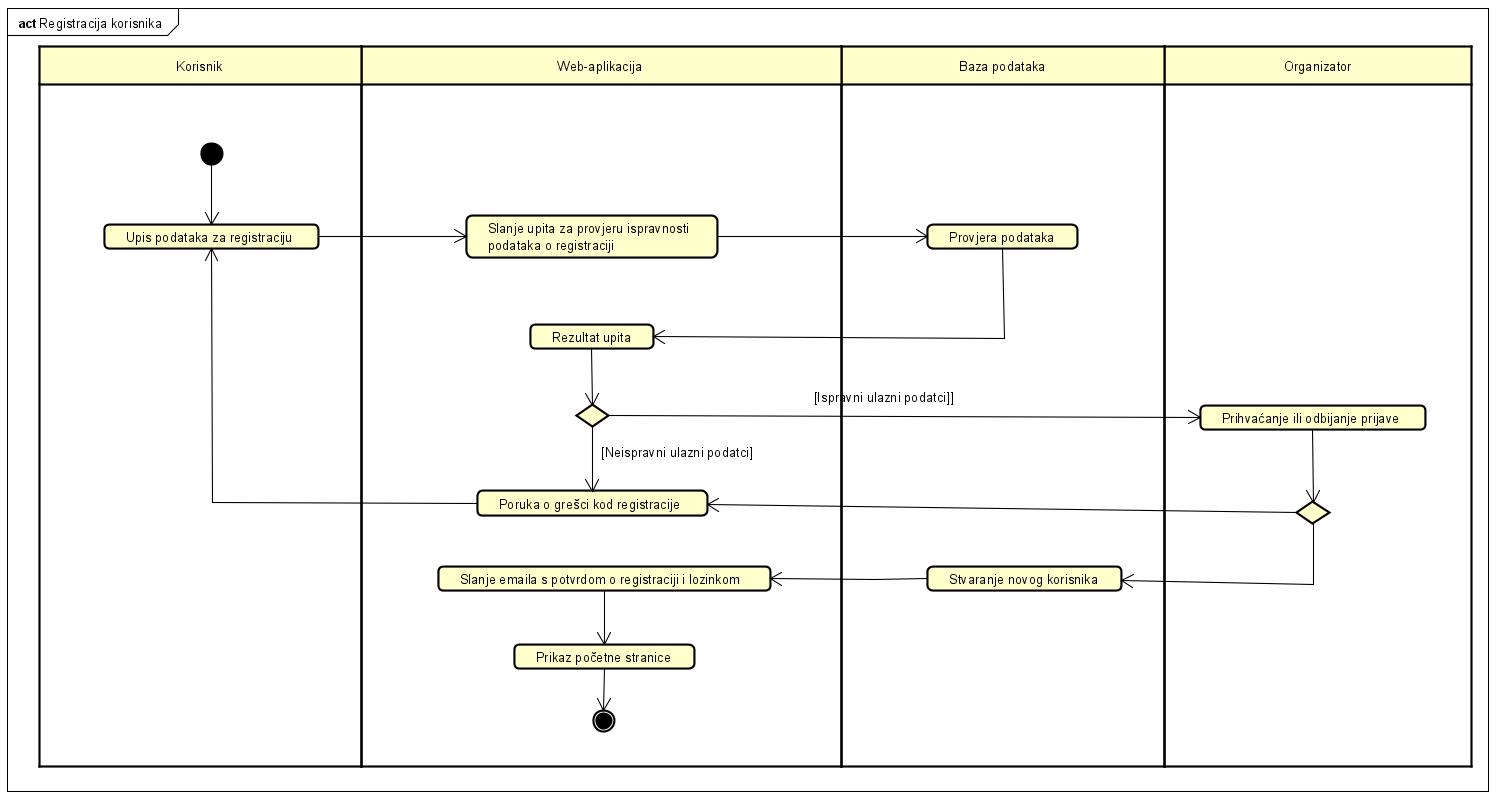
\includegraphics[scale=0.5]{dokumentacija/dijagrami/activity-registracijaKorisnika.PNG} 
	\centering
	\caption{Rregistracija korisnika}
	\label{fig:promjene}
\end{figure}

\begin{figure}[H]
	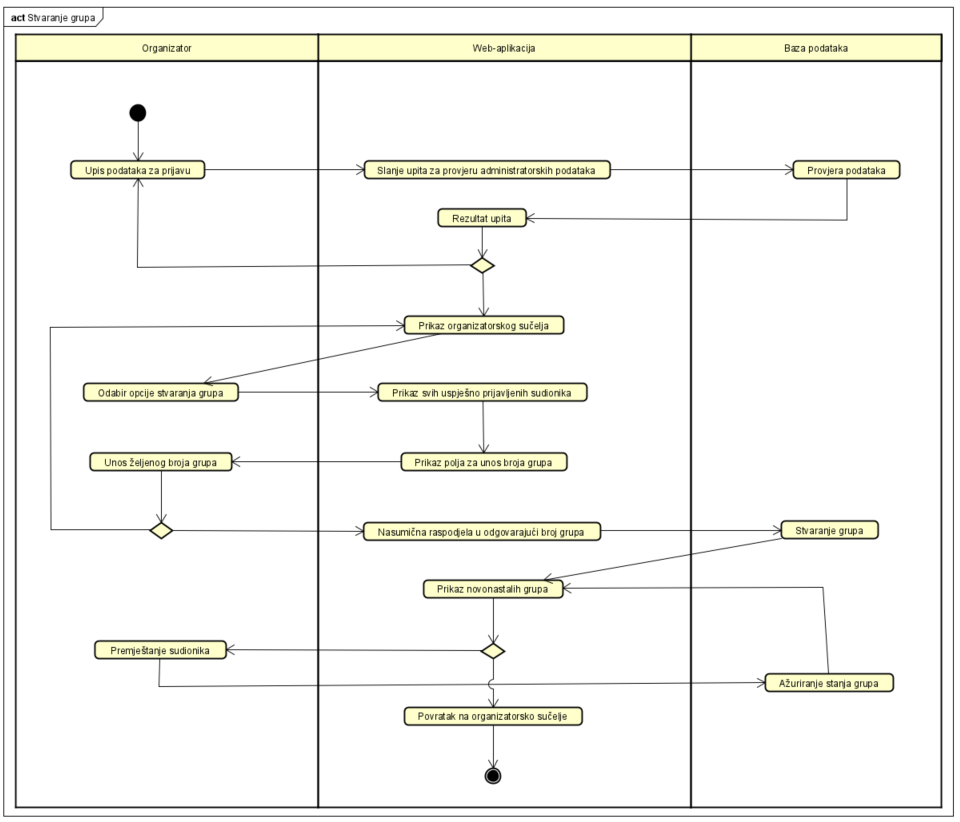
\includegraphics[scale=0.8]{dokumentacija/dijagrami/activity-stvaranjeGrupa.PNG} 
	\centering
	\caption{Stvaranje grupa}
	\label{fig:promjene}
\end{figure}

\eject
\section{Dijagram komponenti}

\begin{figure}[H]
	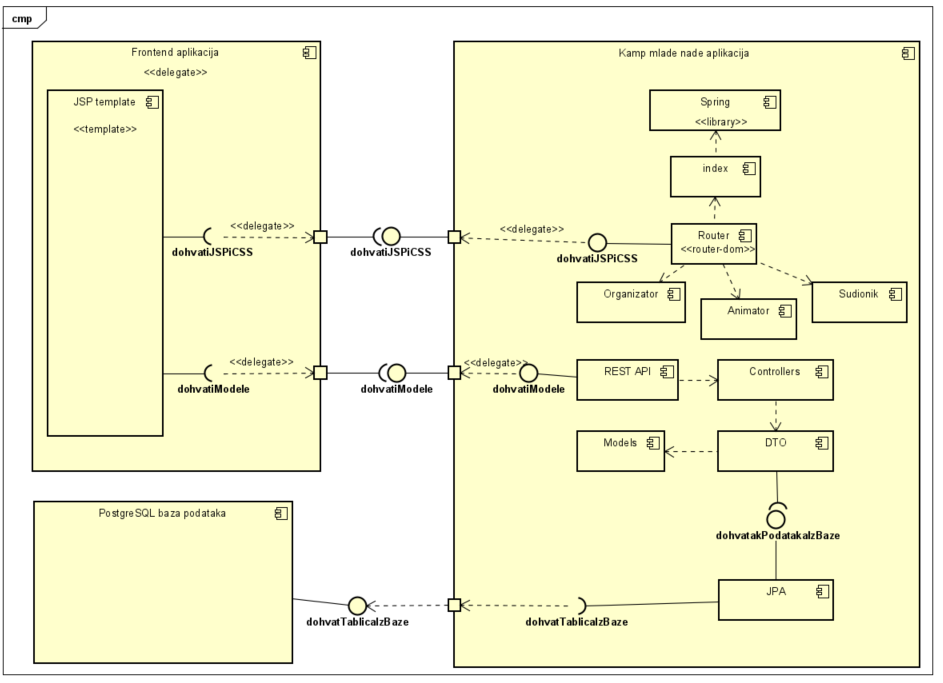
\includegraphics[scale=0.8]{dokumentacija/dijagrami/dijagramKomponenti.PNG} 
	\centering
	\caption{Dijagram komponenti}
	\label{fig:promjene}
\end{figure}
